% !TEX encoding = UTF-8 Unicode
% $Header: /cvsroot/latex-beamer/latex-beamer/solutions/conference-talks/conference-ornate-20min.en.tex,v 1.6 2004/10/07 20:53:08 tantau Exp $

\documentclass{beamer}

\mode<presentation>
{
  \usetheme{Warsaw}
  % or ...

  \setbeamercovered{invisible}
  % or whatever (possibly just delete it)
  
  \setbeamertemplate{navigation symbols}{}
  
  \newcommand*\oldmacro{}%
  \let\oldmacro\insertshorttitle%
  \renewcommand*\insertshorttitle{%
    \oldmacro\hfill%
    \insertframenumber\,/\,\inserttotalframenumber}
}

\usepackage[utf8]{inputenc}
% or whatever

\usepackage{times}
\usepackage{multirow}
\usepackage[T1]{fontenc}
\usepackage[french]{babel}
\usepackage{graphicx}

\usepackage{eso-pic}
\usepackage{color}
\usepackage{tikz}
\usepackage{wasysym}

% Or whatever. Note that the encoding and the font should match. If T1
% does not look nice, try deleting the line with the fontenc.

%\title[Petit guide des bonnes pratiques pour la construction et la maintenance d'$\alpha$-extracteurs cosmiques à vacuité]
{}

\titlegraphic{\raisebox{2em}{}}

\author[Prologin]
{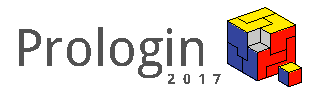
\includegraphics{../prologin2017}}

\date
{}

\begin{document}

\definecolor{vert}{rgb}{0.07 0.54 0.07}


\begin{frame}
        \centering 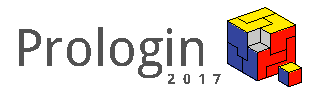
\includegraphics[width=0.9\linewidth]{../prologin2017} \\
        \vspace{1.5cm}
    \textbf{Tabula Prologina}
    \vspace{0.5cm}

    \textit{Felix qui potuit cognoscere algorithmum}
\end{frame}

\begin{frame}
    \frametitle{Qui sommes nous?}
    \begin{itemize}
        \item Alchimistes éminents du XVIII\ieme{} siècle
        \item À la recherche du prochain Grand Maître
        \item Il est présent parmis \textbf{vous}!
    \end{itemize}
\end{frame}

\begin{frame}
    \frametitle{Présentation de l'épreuve d'alchimie}
    \begin{itemize}
        \item Deux apprentis travaillent simultanément sur leurs établis
        \item Chacun tente de transmuter ses éléments en or
        \item Celui qui possède le plus d'or est le plus Grand des deux
    \end{itemize}
\end{frame}

\begin{frame}
    \frametitle{Votre espace de travail}
    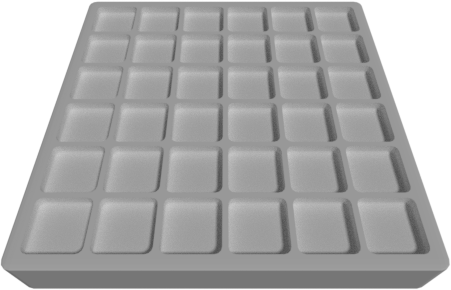
\includegraphics[width=\textwidth]{../img/bench-empty}
\end{frame}

\begin{frame}
    \frametitle{Échantillon}
    \begin{block}{Éléments}
        \begin{tabular}{ccccc}
            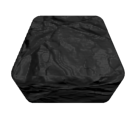
\includegraphics[width=1.5cm]{../img/material-lead} &
            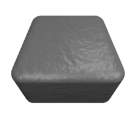
\includegraphics[width=1.5cm]{../img/material-iron} &
            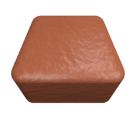
\includegraphics[width=1.5cm]{../img/material-copper} &
            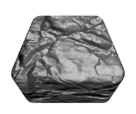
\includegraphics[width=1.5cm]{../img/material-mercury} &
            
\includegraphics[width=1.5cm]{../img/material-sulfur}\\
            Plomb & Fer & Cuivre & Mercure & Soufre
        \end{tabular}
    \end{block}
    \begin{block}{Échantillon}
        Constitué de deux éléments, identiques ou différents.
    \end{block}
    \begin{block}{Placement d'un échantillon}
        \begin{itemize}
            \item Éléments posés sur des cases adjacentes
            \item Un des deux éléments doit être posé adjacent à un élément du
                même type déjà sur l'établi
            \item Si aucun des deux éléments n'est présent, placement libre
        \end{itemize}
    \end{block}
\end{frame}

\begin{frame}
    \frametitle{Donner un échantillon}
    \begin{block}{Choisi pour l’adversaire}
        \begin{itemize}
            \item On ne se sert pas soi-même dans la réserve!
            \item On apporte un échantillon à son camarade
            \item Au tour $N$, choisi l'échantillon du tour $N + 1$ de
                l'adversaire
        \end{itemize}
    \end{block}
    \begin{block}{Contraintes}
        L'échantillon donné doit avoir au moins un élément en commun avec
        l'échantillon reçu.
    \end{block}
    \begin{block}{Oubli}
        Si vous oubliez de donner un échantillon à votre adversaire, il recevra
        la même chose que ce qu’il vous a donné au tour précédent.
    \end{block}
\end{frame}

\begin{frame}
    \frametitle{Transmutation}
    \begin{block}{Transmutation forte}
        Transforme \textbf{cuivre}, \textbf{fer} ou \textbf{plomb}, en or.
        \\
        \begin{tabular}{ccccc}
            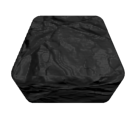
\includegraphics[width=1.5cm]{../img/material-lead} &
            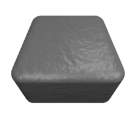
\includegraphics[width=1.5cm]{../img/material-iron} &
            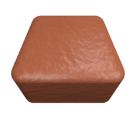
\includegraphics[width=1.5cm]{../img/material-copper} &
            $\xrightarrow{\text{transmutation}}$ &
            
\includegraphics[width=1.5cm]{../img/material-gold}\\
            Plomb & Fer & Cuivre & & Or
        \end{tabular}
    \end{block}
    \begin{block}{Transmutation faible}
        Transforme \textbf{soufre} ou \textbf{mercure} en catalyseur
        \\
        \begin{tabular}{cccccc}
            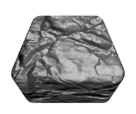
\includegraphics[width=1.5cm]{../img/material-mercury} &
            
\includegraphics[width=1.5cm]{../img/material-sulfur} &
            $\xrightarrow{\text{transmutation}}$ &
            
\includegraphics[width=1.5cm]{../img/material-catalyst} &
            + &
            
\includegraphics[width=0.5cm]{../img/material-gold}\\
            Mercure & Soufre & & Catalyseur & & Or\\
        \end{tabular}
    \end{block}
\end{frame}

\begin{frame}
    \frametitle{Effectuer une transmutation}

    \begin{block}{Zone d'application}
        \begin{itemize}
            \item Tout une zone d'éléments du même type adjacent.
            \item Impossible de sélectionner une sous-zone
            \item Disparaît après transmutation
        \end{itemize}
    \end{block}
    \begin{block}{Points}
        Une zone de taille $t$ rapporte $-3$ d'or si $t = 1$, sinon:
        \begin{itemize}
            \item forte: $\lfloor \frac{t^2}4 \rfloor - 1$ d'or
            \item faible: $t - 2$ d'or et
                $\lfloor \frac{t-1}2 \rfloor$ catalyseurs
        \end{itemize}
        \begin{tabular}{l|c|c|c|c|c|c|c|c|c|c|c}
            Taille & 1 & 2 & 3 & 4 & 5 & 6 & 7 & 8 & 9 & 10 & ..\\
            \hline
            Or (forte)   & -3 & 0 & 1 & 3 & 5 & 8 & 11 & 15 & 19 & 24 & ..\\
            \hline
            Or (faible)  & -3 & 0 & 1 & 2 & 3 & 4 & 5  & 6  & 7  & 8  & ..\\
            \hline
            Catalyseurs     & 0  & 0 & 1 & 1 & 2 & 2 & 3  & 3  & 4  & 4  & ..
        \end{tabular}
    \end{block}
\end{frame}

\begin{frame}
    \frametitle{Catalyse}
    \vspace{1cm}
    \begin{tabular}{ccccccc}
        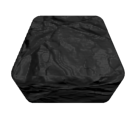
\includegraphics[width=0.8cm]{../img/material-lead} &
        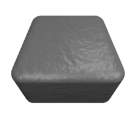
\includegraphics[width=0.8cm]{../img/material-iron} &
        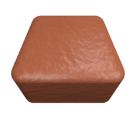
\includegraphics[width=0.8cm]{../img/material-copper} &
        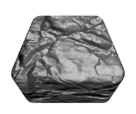
\includegraphics[width=0.8cm]{../img/material-mercury} &
        
\includegraphics[width=0.8cm]{../img/material-sulfur} &
        $\xrightarrow{\text{Catalyse}}$ &
        
\includegraphics[width=0.8cm]{../img/material-other}\\
        Plomb & Fer & Cuivre & Mercure & Soufre &
        
\includegraphics[width=0.5cm]{../img/material-catalyst} &
        Élément
    \end{tabular}

    \vspace{1cm}
    \begin{itemize}
        \item Un catalyseur transforme un métal vil en un autre
        \item La réaction peut être déclenchée chez l’adversaire!
    \end{itemize}
    \begin{alertblock}{Attention}
        Un catalyseur est instable et doit être utilisé immédiatement
    \end{alertblock}
\end{frame}

\begin{frame}
    \frametitle{Déroulement d’une partie}
    \begin{block}{Nombre de tours}
        \begin{itemize}
            \item 150 tours
            \item Un apprenti joue les tours pairs, l'autre les impairs
        \end{itemize}
    \end{block}
    \begin{block}{Actions}
        Les actions possibles sont (sans ordre):
        \begin{itemize}
            \item Poser son échantillon: 1 fois, \textbf{obligatoire}
            \item Donner un échantillon pour l'adversaire: 1 fois
            \item Transmuter: autant de fois que voulu
            \item Catalyser: autant de fois que de catalyseurs disponibles
        \end{itemize}
    \end{block}
    \begin{alertblock}{Poser l'échantillon est obligatoire}
        Échantillon non posé $\rightarrow$ établi entièrement vidé!
    \end{alertblock}
\end{frame}

\begin{frame}
    \frametitle{Questions}
    Posez vos questions sur le sujet de la finale!
\end{frame}

\begin{frame}
    \frametitle{Tournois intermédiaires}
    \begin{itemize}
        \item Samedi 15~h~42 (tournoi test)
        \item Samedi 17~h~42
        \item Samedi 23~h~42
        \item Dimanche 5~h~42
        \item Dimanche 11~h~42
        \item Dimanche 17~h~42
        \item Lundi 00~h~42 (tournoi final)
    \end{itemize}
\end{frame}

\begin{frame}
    \frametitle{Conférences}
    \begin{itemize}
        \item \textbf{Samedi 16~h} Antoine Amarilli : Qu'est-ce que
            l'informatique théorique et comment en faire?
        \item \textbf{Lundi 11~h~30} Éva Attal : Les métiers de développeurs en
            salle de marché
    \end{itemize}
\end{frame}

\begin{frame}
    \frametitle{Fin}
    Bonne finale !
\end{frame}

\end{document}
